\section{Tool Flow}\label{sec:flow}

While constructing the e-graph is the crux of \shortname{}, there are several
other important components to consider in the full design flow. In order to
test our hypothesis, \shortname{} must be compatible with existing synthesis
flows, and attempts at finding reduced circuits must be verified.

\begin{figure}
    \begin{subfigure}{0.47\textwidth}
        \centering
        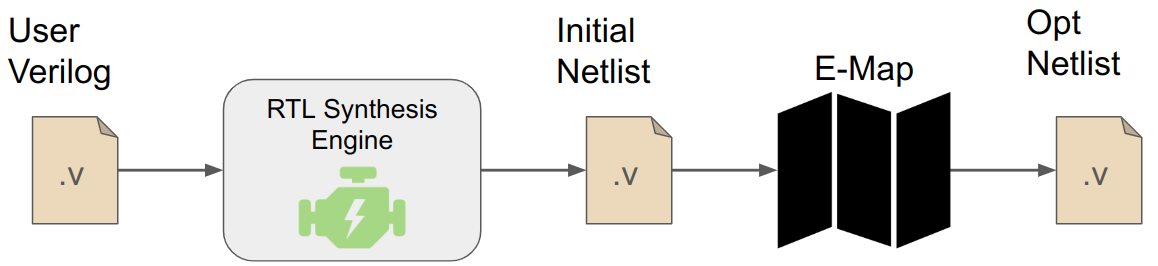
\includegraphics[width=\textwidth]{img/flow.png}
        \caption{Tool flow to integrate E-Pack with existing RTL synthesis engines.}\label{fig:flow:rtl}
        \Description[]{}
    \end{subfigure}
    \hfill\vspace{4mm}
    \begin{subfigure}{0.47\textwidth}
        \centering
        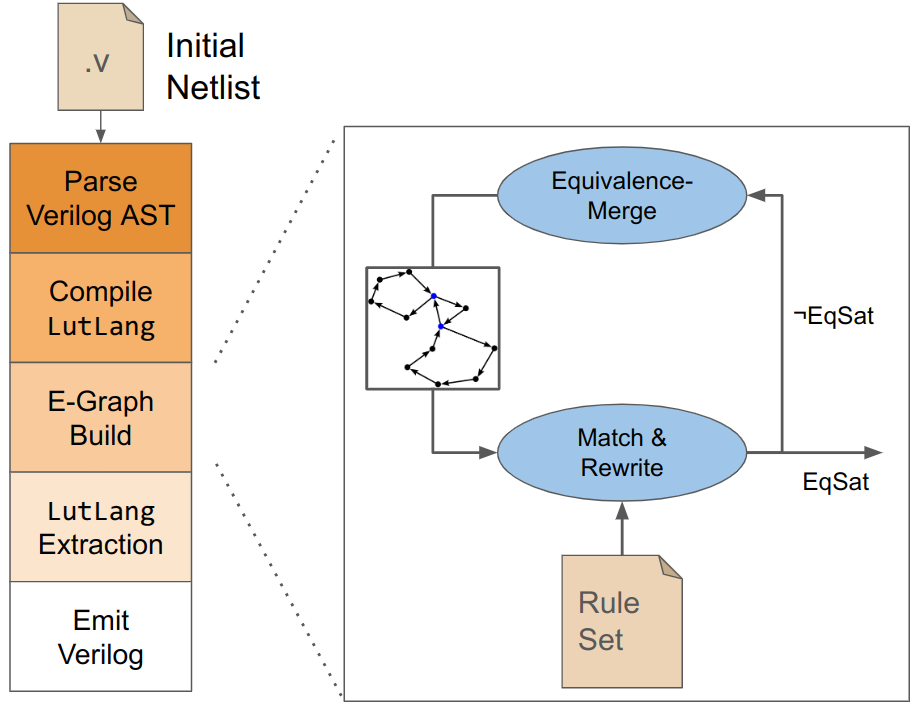
\includegraphics[width=\textwidth]{img/egraph.png}
        \caption{Compilation steps internal to \shortname{} Verilog tool.}\label{fig:flow:egraph}
        \Description[]{}
    \end{subfigure}
    \caption{\todo{root caption}}\label{fig:flow}
\end{figure}

\subsection{Extraction}\label{sec:flow:extraction}
Regardless of whether equality saturation is achieved or not, the quality of
the output circuit still largely depends on the extraction technique used. In
short, \textit{extraction} is the process of selecting the ``best'' circuit
from the e-graph. Given that a saturated e-graph can contain hundreds of
thousands of e-nodes across tens of thousands of e-classes, a greedy extraction
algorithm is the most pragmatic. The greedy extractor iterates over the
e-classes, updating the cost of the cheapest e-node until the database of costs
no longer change. Whenever possible, our compiler uses the builtin
functionality of the egg e-graph Rust library~\cite{docsEgg}. However, e-graph
extraction itself is an ongoing research area~\cite{smoothe,
    sparsextract,esynth}, and future work would experiment with different
extraction algorithms. In any case, the cost of a LUT is always one plus the
sum of the costs of its children nodes. The subtle interactions between
extraction and the rewrite rule set are further explained in
Section~\todo{result sec}.

\subsection{Verilog Support}\label{sec:flow:verilog}
In order for our compiler to be compatible with as many existing design flows
as possible, some level of Verilog support is necessary. Our compiler supports
an ad-hoc subset of Verilog 2001~\cite{verilog}, as required to represent
structural netlists. This includes support for non-ANSI C style module
delcarations, wires, and module instantiations with named port connections.
With Verilog support, we are able to test \shortname{} with tool flows that use
Yosys~\cite{yosys} or Vivado~\cite{vivado}. On the backend, our compiler also
emits an updated Verilog netlist.

\subsection{Verification}\label{sec:flow:verification}
While verification is the not the primary focus of this work, some level of
validation is required to build trust in our synthesis results. In fact,
e-graphs were originally designed for automated theorem
proving~\cite{eggpaper}. Thus, constructing proofs that demonstrate equivalence
between the original and optimized netlist is a builtin feature of
\shortname{}. However, this technique is relatively slow, so we use two other
independent sources of verification. For combinational netlists, our middle end
can do exhaustive functional testing. Lastly, we use Yosys~\cite{yosys} for its
SAT-driven equivalence checking capabilities. All in all, the mixed usage of
these verification techniques build great confidence in the robustness of our
technology mapper built around e-graphs.